\documentclass{article}
\usepackage{fontspec}
\usepackage{jim}
\usepackage{amsmath}
\usepackage[french]{babel}
\usepackage{listings}
\usepackage{diagbox}
\usepackage{caption}
\usepackage{booktabs}
\usepackage{microtype}
%\usepackage{pxfonts}
\usepackage{graphicx}
\usepackage{hyperref}
\usepackage{tikz}
\usepackage{xspace}
\setmainfont{Tribun ADF Std}
\usepackage{array}

\newcolumntype{C}[1]{>{\centering\arraybackslash}m{#1}}   %% centered
\newcolumntype{R}[1]{>{\raggedright\arraybackslash}m{#1}}  %% right aligned
\newcolumntype{L}[1]{>{\raggedleft\arraybackslash}m{#1}}  %% right aligned

\newcommand\trigger{point d'interaction\xspace}
\newcommand\triggers{points d'interaction\xspace}
\newcommand\vocab[1]{\textbf{#1}}
\DeclareCaptionType{scenario}[Scénario]
% Title.
% ------
\title{Écriture et exécution répartie de scénarios interactifs}

\threeauthors
  {Auteur 1} {Organisme \\ Adresse électronique}
  {Auteur 2} {Organisme \\ Adresse électronique}
  {Auteur 3} {Organisme \\ Adresse électronique}

\begin{document}
\maketitle
\begin{abstract}
    La pratique musicale est souvent une opportunité pour interagir et échanger, 
    avant tout avec d'autres musiciens, et plus récemment avec des algorithmes ou logiciels 
    disposant d'un certain degré d'autonomie et de liberté.
    
    La notation musicale occidentale résout le problème du partage d'information entre musiciens 
    en séparant une partition en portées; la plupart des logiciels musicaux vont interpréter cette 
    portée sur une seule machine, en gardant la possibilité de pistes avec des réglages indépendants. 
    
    Ce document présente d'une part une généralisation de cette notion de partage aux scénarios interactifs, 
    et d'autre part une implémentation pratique dans le logiciel i-score, mettant en valeur 
    les possibilités d'écriture augmentées qu'offre une exécution répartie à un compositeur.
\end{abstract}
\section{Problématique}
On cherche à définir une sémantique permettant de décrire l'exécution d'une partition interactive sur plusieurs machines, en prenant en compte les exécutions parallèles, c'est-à-dire que deux machines jouent la même chose, de manière synchronisée ou non, ainsi que les exécutions série : une machine joue puis une autre machine joue la suite.

On parle ici de «jeu» à un niveau abstrait~: on s'intéresse au contrôle de tous types de paramètres et non pas uniquement les paramètres musicaux.

On présentera d'abord plusieurs applications et problématiques pratiques rencontrées par des artistes et auteurs, qui ont motivé ce travail.
Puis, les possibilités de répartition étudiées seront présentées dans le détail, en analysant l'impact que peuvent avoir les problèmes connus dans le domaine de l'informatique répartie, sur l'écriture de telles partitions. Pour conclure, les performances du système développé seront présentées.

\section{Études de cas}
-> installation en son réparti ?

- Problème de la latence entre i-score et raspberry, + utilisation de bande passante.

- Cas des applis de téléphone : un objet qui s'exécute sur plusieurs machines en parallèle dont on veut aggréger les résultats

- Donner la possibilité de faire un dialogue (boucle avec un coup un \trigger qui vient de A, un coup un \trigger qui vient de B, etc)

- Approche alternative avec application mobile.

- Faciliter l'écriture de programmes qui s'exécutent sur des machines embarquées

- Lister les cas. D'abord non interactif (partage uniquement des processus), puis interactif.

On veut : résistance aux "normal" failures, pas Byzantine failures.
\subsection{État de l'art}
\subsubsection{Rappel du modèle d'i-score}
Vocabulaire. Prendre article SMC.

Ici les processus de donnés sont représentés par une boite barrée en diagonale (cas courant d'une courbe montante).

Mettre accent sur hiérarchie
%\subsubsection{Répartition à l'édition}
\subsubsection{Répartition à l'exécution}
%\subsubsection{Lien entre la répartition à l'édition et la répartition à l'exécution}

- Problème des devices. Note : si on se permet d'envoyer des messages OSC quelconques (i.e. pas dans l'arbre), ça peut simplifier des choses. Aussi, permettre devices qui sont juste en mode envoi ? Il faut un autre proto que OSC ou Minuit...

Aussi, refactoriser pour utiliser tout i-score en librairie

\subsubsection{Horloges}
Problème de l'horloge : 
\begin{itemize}
\item Si on utilise l'horloge système, pas de garantie qu'elle soit bien synchronisée. 
Et NTP pas dispo partout (on n'a pas forcément les droits sur un téléphone pour changer l'heure).
Horloge i-score se resynchronise déjà en cas de délai sur une machine.
\item Si on utilise une horloge interne, problème de la synchronisation avec l'horloge système (pour le tick)
\end{itemize}

\url{http://queue.acm.org/detail.cfm?id=2745385}
\url{http://radar.oreilly.com/2012/10/google-spanner-relational-database.html}
\url{http://www.ntp.org/ntpfaq/NTP-s-sw-clocks-quality.htm}

Faire la relation entre notre système et le problème CAP : \url{https://en.wikipedia.org/wiki/PACELC_theorem}

Horloges logiques : équivalent à envoyer une timestamp à chaque tick (on arrive donc à un méchanisme de vector clock approximatif). 

Synchro d'horloges de deux machines dont une qui ralenti, si elles exécutent le même 
scénario ? Il faut les recaler régulièrement. 

Possibilité : externe (NTP, etc) ou interne : \url{https://github.com/ethanlim/NetworkTimeProtocol}

Recaler dès qu'on accumule du retard ?



On peut introduire un recalage sur la master clock entre chaque tick.

Ce qu'on fait : ping régulier vers chaque client (toutes les 100 millisecondes)

Quand quelque chose doit se synchroniser, on dit à chaque machine à quel instant il est supposé arriver par rapport à son horloge système.

Quand un client reçoit un ordre pour un timenode à t, il l'applique dès que t <= local(t) (modulo un tick?)



Possibilité : synchronisation via démon externe (PTP, NTP...), mais pas toujours possible (on ne peut pas supposer que l'utilisateur a les droits pour changer l'horloge sur sa machine).

Synchronous ethernet

Ableton Link : synchro sur les ticks musicaux 

Avoir une horloge propre à i-score ? Mais du coup maintenant il faut la synchroniser à l'horloge système. 

\subsubsection{Problématique de la sécurité}

\subsubsection{Synchronisation de médias}
- pas pour l'instant... doivent être au même endroit sur la même machine.
Ableton Link ? Netjack ?

\section{Approche}
Cette section détaille les choix de haut niveau réalisés.

On souhaite modifier le moins possible le modèle pour les utilisateurs du logiciel, 
en rajoutant les notions nécessaires et suffisantes pour offrir la finesse de répartition désirée.

La section~\ref{sec.description} présente de manière détaillée les possibilités 
de répartition que l'on offre, en prenant example sur des cas simples.

La section~\ref{sec.semantique} définit ces possibilités en utilisant les objets du modèle d'i-score.

Enfin, la section~\ref{sec.evaluation} présente une évaluation des performances dans le cadre 
d'une implémentation pratique.

\subsection{Nouvelles notions}
Nous nous trouvons en présence de plusieurs machines qui communiquent et partagent un document.
L'ensemble constitué par les instances d'i-score et le document qu'elles partagent est appelé \vocab{session}.

On désigne par \vocab{client} une instance d'i-score connectée à une session.

On désire s'affranchir des notions propres aux machines physiques et des problématiques de réseau (addresse IP, etc) lors de l'écriture 
d'un scénario réparti. 

Pour ce faire, on introduit la notion de \vocab{groupe}. 
Un groupe est un ensemble de clients.

Les compositeurs ne travaillent manipulent jamais directement la notion de client, uniquement celle d'un groupe qui peut contenir zéro, un, ou plusieurs clients.

De manière générale, quand plusieurs clients font partie d'un même groupe, cela signifie qu'ils vont réaliser les mêmes tâches, de manière synchrone ou asynchrone.

L'intérêt d'un groupe est la tolérance aux pannes, déconnections, reconnections, et changements d'installation. 
Par exemple, si une machine tombe en panne, on peut la remplacer par une autre simplement en l'assignant au même groupe que la machine en panne 
sans avoir besoin de mettre à jour le scénario.

\begin{figure}[h]
	\centering
	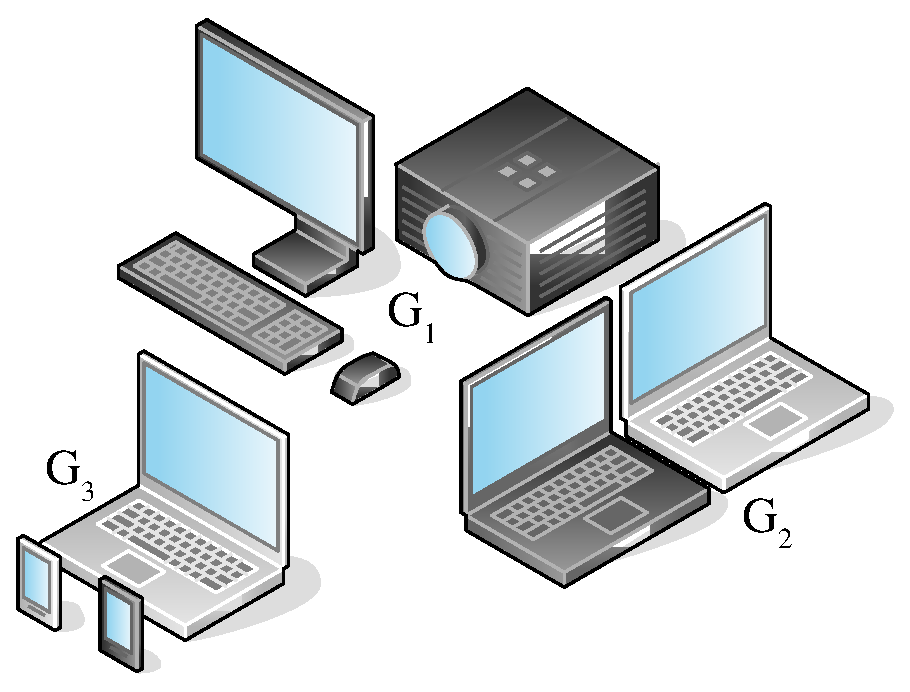
\includegraphics[scale=0.2]{images/groupes.eps}
	\caption{Plusieurs groupes avec plusieurs machines dans chaque groupe}
	\label{img.groupes}
\end{figure}


\subsection{Topologie}
Maître-esclave pour l'édition.

Pour des raisons de simplicité, la première mise en œuvre se fait via une toplogie réseau en étoile : un maître gère 
le déroulement général de l'exécution. 
Les différents clients communiquent au travers de ce maître, avec les avantages et inconvénients que cela implique : 
\begin{itemize}
	\item Facilité d'analyse lors du développement : on peut enregistrer tous les messages échangés avec leurs estampilles.
	\item Intolérance aux pannes : si le maître faillit, aucune récupération n'est possible.
\end{itemize}

On détaille dans les sections suivantes les cas ou des topologies différentes peuvent montrer un intérêt.

Pour l'exécution : dans certains cas deux machines peuvent échanger directement.
Il faut décrire ces cas.

Si groupes avec plusieurs machines : "group leader" ? responsable de la communication ? avoir un "plus court chemin" permanent ?

\subsection{Fondements}
Première approche basées sur réseau de Petri.

Puis migration du modèle d'i-score maintenant autonome.

Il est possible d'implément ce méchanisme de répartition purement avec les primitives dont on dispose dans i-score, 
mais c'est prohibitoire pour les utilisateurs.

Différentes possibilités de répartition sont disponibles selon les types de processus.

Détailler les implications des choix par rapport au théorême CAP et PACELT.
\subsection{Modèle}
i-score se base sur une approche orientée document.

On choisit de répartir nos objets autour d'un même document partagé par toutes les instances du réseau, 
à la manière des logiciels d'édition tels que Google Docs. %CITE

Cela ne pose pas de problème de mémoire, même sur de l'embarqué : 
les scénarios i-score sont très compacts (en général quelques dizaines de kilo-octets).

\subsection{Répartition de l'édition}
- Partage de file undo - redo. Transformations opérationnelles. %CITE

- Autres approches : partage du modèle lui-même.

\section{Description de l'exécution}\label{sec.description}
On sépare les objets offrant une structure temporelle, des objets possédant des données (par exemple, une automation).
\subsection{Processus de contenu}
On entend par processus de contenu, tous les processus produisant des données, sans se soucier de la structuration temporelle. En voici une liste non exhaustive : automation, mapping, code javascript, piano roll MIDI, audio\dots

Le processus s'exécute tel quel pour toutes les machines auquel il est assigné, 
et ne s'exécute pas pour les autres.

% TODO pour devices, faire en sorte que les clients ne se connectent que à ceux qui sont en local ? Ou même mode "non connecté" (mais impossible de recevoir comme ça). Ou bien avoir une "map" d'addresse ip / port pour chaque paire client <-> device.

\subsubsection{Comportements de groupes}
-> pourquoi ne pas avoir la même chose au niveau des mappings (et pour tout ce qui n'est pas fixé de manière générale ?)
Deux manières : offrir un processus de mapping spécialisé qui permet de définir les relations qu'on veut dans un groupe ("first", "all", "mean", "sum", etc...)

Ou bien faire cette transformation à plus bas niveau (pour les devices) : les sorties sont constantes mais on peut appliquer des transformations aux entrées.

\subsection{Processus Scénario}
Le scénario est le processus central d'i-score : il met en relation les différents éléments temporels.

Plusieurs manières de répartir l'exécution d'un scénario, offrant différentes possibilités d'écriture, sont détaillées ci-dessous. On sépare le cas général permettant l'interactivité dans un scénario (le scénario continue après qu'un évènement externe $e$ se soit déclenché, visible par exemple en scénario~\ref{scenar.general}) du cas plus simple ou les dates sont fixées, visible en scénario~\ref{scenar.non-interactif}.

On travaillera dans les examples suivants avec trois groupes $A,B,C$ disposant chacun d'un nombre inconnu de clients.

\subsubsection{Modes de synchronisation}
On identifie trois niveaux de synchronisation, qui peuvent chacuns avoir leur utilité dans un cas différent : 
\begin{itemize}
    \item Asynchrone : lorsqu'une information interactive est disponible dans le système (par exemple «une expression se vérifie»), elle est propagée le plus vite possible aux autres noeuds qui doivent appliquer le résultat de cette information. Ce mode ne respecte pas nécessairement la sémantique avant-après de i-score mais permet de réduire la latence.
    \item Synchrone : lorsqu'une information est disponible dans le système, elle est propagée de manière à ce que la date absolue de réalisation soit  la même (pour un observateur externe) pour tous les clients. 
    Ce mode respecte la sémantique de i-score~: les éléments s'exécutent dans le même ordre que si le scénario n'était pas réparti, au prix d'une latence augmentée.    
    Il convient de rappeler qu'il est physiquement impossible d'exécuter les objets avec la même précision temporelle que s'ils étaient exécutés dans un même tic d'horloge sur le même client: l'objectif est de minimiser les décalages temporels.
    \item Précalculé : ce mode est surtout utile dans le cas non-interactif : dès qu'une date peut être fixée, elle l'est, et les clients n'attendent pas de message annonçant la fin. 
    Plus la synchronisation des horloges sera fine entre les clients et plus ce mode se rapprochera de l'exécution dans le cas non réparti.
\end{itemize}

Les différents modes de synchronisation vont impacter : 
\begin{itemize}
    \item L'exécution des \triggers.
    \item La vérification de la validité des conditions.
    \item Le changement de vitesse d'exécution des contraintes temporelles.
\end{itemize}

Lorsqu'un choix doit être fait, un consensus peut être pris au niveau du groupe auquel est assigné l'objet. 
Par exemple, quelle va être la vitesse à laquelle une contrainte temporelle va s'exécuter.
Les mécanismes de consensus possibles sont détaillés plus en détail par la suite.

\subsubsection{Cas interactif}
Trois niveaux de partage : 

\begin{itemize}
    \item Partage complet : il n'y a qu'une seule ligne temporelle partagée pour toutes les machines. 
    Les annotations de machines indiquent l'emplacement d'exécution. 
    Les groupes servent à indiquer ou non l'exécution d'un processus sur une machine et le groupe devant parvenir à un consensus pour une expression donnée. 
    Si par exemple la vitesse d'exécution d'une contrainte est modifiée en temps réel, cette modification est répercutée sur toutes les machines.
    
    Cela permet notamment de gérer la répartition d'objets à des niveaux hiérarchiques différents~: dans le scénario~\ref{scenar.hierarchy}, si le scénario racine est dans ce mode, alors on peut correctement faire exécuter les scénarios enfants en prenant en compte les groupes de leurs objets. 
    
    \begin{figure}[h]
        \centering
        \begin{tabular}{L{3.5em}R{0.3\textwidth}}
            Racine: & \begin{tikzpicture}
            \input{scenarios/hierarchy.tex}
            \end{tikzpicture} \\
            $S_1$: & \begin{tikzpicture}
            \input{scenarios/hierar-sub.tex}
            \end{tikzpicture} \\
            $S_2$: & \begin{tikzpicture}
            \input{scenarios/hierar-sub-2.tex}
            \end{tikzpicture} \\
        \end{tabular}
        \captionof{scenario}{Deux contraintes possédant chacune un scénario hiérarchique}
        \label{scenar.hierarchy}
    \end{figure}
    
    \item Aucun partage : les machines n'étant pas associées à ce processus ne l'exécutent pas, celles qui y sont associées l'exécutent toutes de manière indépendante.
    Si par exemple on assigne le groupe $A$ au scénario~\ref{scenar.general}, tous les clients de $A$ vont exécuter tous les éléments, sans communiquer sur leurs résultats. 
    Par exemple, pour deux machines $A_1$ et $A_2$, le \trigger pourra se déclencher à des instants différents, et la condition pourra avoir une valeur différente.
    Cela implique que les groupes assignés aux objets du scénario soient ignorés, récursivement : puisque chaque exécution va avoir des temps différents par conception, il ne peut pas y avoir de synchronisation.
    
    Ce cas est notamment utile pour avoir des sous-scénarios dont plusieurs participants à une installation artistique peuvent faire l'expérience en même temps, tout en gardant une trame générale de plus haut niveau. 
    Typiquement, on peut imaginer ce cas pour une application mobile.
    
    \begin{figure}[h]
        \centering
        \begin{tikzpicture}
        \fill (0, 18.7148) circle (0.075) ; % State.0 
\fill (2.15596, 18.7148) circle (0.075) ; % State.1 
\fill (2.15596, 17.4029) circle (0.075) ; % State.2 
\fill (4.40367, 17.4029) circle (0.075) ; % State.3 
\fill (0, 18.0053) circle (0.075) ; % State.4 
\fill (2.15596, 18.0187) circle (0.075) ; % State.5 
\fill (2.15596, 16.7068) circle (0.075) ; % State.6 
\fill (5, 16.7068) circle (0.075) ; % State.7 
\draw[line width=1pt] (0, 18.7148)  -- (0, 18.0053) ; % TimeNode.0 
\draw[line width=1pt] (2.15596, 18.7148)  -- (2.15596, 16.7068) ; % numb47vine94 
\draw (2.15596, 18.9648) node {$C$}; % numb47vine94 
\draw[line width=1pt] (4.40367, 17.4029)  -- (4.40367, 17.4029) ; % faze44greg1 
\draw[line width=1pt] (5, 16.7068)  -- (5, 16.7068) ; % burp79lawn67 
\draw[line width=1pt] (0, 18.7148)  -- (1.39908, 18.7148) ; % dido10rend91 
\draw[dashed,line width=1pt] (1.39908, 18.7148)  -- (2.86239, 18.7148) ; % dido10rend91 
\draw[line width=0.7pt] (1.63908, 18.8678) arc(90:270:0.15) ; % dido10rend91 
\draw[line width=0.7pt] (2.71239, 18.5648) arc(-90:90:0.15) ; % dido10rend91 
\draw (1.07798, 18.9148) node {$A$}; % dido10rend91 
\draw[line width=1pt] (2.15596, 17.4029)  -- (4.40367, 17.4029) ; % taut8hews94 
\draw (3.27982, 17.6029) node {$D$}; % taut8hews94 
\draw[line width=1pt] (0, 18.0053)  -- (1.38073, 18.0053) ; % ramp48lust85 
\draw[dashed,line width=1pt] (1.38073, 18.0053)  -- (2.90826, 18.0053) ; % ramp48lust85 
\draw[line width=0.7pt] (1.62073, 18.1583) arc(90:270:0.15) ; % ramp48lust85 
\draw[line width=0.7pt] (2.75826, 17.8553) arc(-90:90:0.15) ; % ramp48lust85 
\draw (1.07798, 18.2053) node {$B$}; % ramp48lust85 
\draw[line width=1pt] (2.15596, 16.7068)  -- (5, 16.7068) ; % dirt50gage22 
\draw (3.57798, 16.9068) node {$E$}; % dirt50gage22 
\draw[line width=1pt] (1.95596, 16.7068)  -- (1.95596, 16.7068) ; % sill78hues28 
\draw[line width=1pt] (1.95596, 16.7068) arc(180:75:0.2) ; % sill78hues28 
\draw[line width=1pt] (1.95596, 16.7068) arc(180:285:0.2) ; % sill78hues28 

        \end{tikzpicture}
        \captionof{scenario}{Un scénario interactif avec des interactions et des conditions ; $A,B,C,D,E$ sont les groupes associés aux éléments du modèle. On suppose l'existence de processus de contenus dans chaque contrainte temporelle.}
        \label{scenar.general}
    \end{figure}

    \item Partage partiel : il peut y avoir plusieurs lignes temporelles dans un même scénario qui peuvent se resynchroniser à un instant donné. 
    Les annotations donnent l'emplacement d'exécution, et de vérification des expressions. 
    Une machine ne sait pas à l'avance si elle va pouvoir se déclencher ou non. 
    
\end{itemize}



\subsubsection{Cas non-interactif}
% Cas principalement développé dans rapport de master
On peut soit utiliser les méthodes de synchronisation décrites précédemment, mais une possibilité s'ajoute : 

Comme on connait les dates effectives auxquelles les objets sont sensés s'exécuter, on peut les fixer à l'avance sur chaque machine. 
Un parcours de graphe permet d'obtenir une estimation des dates minimales auxquelles il est possible de fixer des dates d'exécutions des éléments suivant un point d'interaction donné.
Le même mécanisme a été utilisé dans~\cite{celerier2016rethinking} pour spécifier les dates d'exécution et de fin de flux audios.


\begin{itemize}
\item Avantage : s'il y a une déconnexion, l'exécution va continuer à fonctionner au moins jusqu'au prochain \trigger.
\item Inconvénient : il suffit d'un peu de délai pour que le début de B survienne avant la fin de A. 
Il est particulièrement important dans ce cas de garder les horloges synchronisées.
\end{itemize}

On notera que modifier la vitesse d'exécution des éléments en temps réel implique de mettre à jour les estimations de dates sur toutes les autres machines. 
En autorisant cela, on pert donc une certaine tolérance au partitionnement.

\begin{figure}[h]
	\centering
	\begin{tikzpicture}
	\input{scenarios/non-interactif.tex}
	\end{tikzpicture}
	\captionof{scenario}{Les groupes A, B, C exécutent des contraintes temporelles à la suite les uns des autres}
	\label{scenar.non-interactif}
\end{figure}


\subsubsection{Expressions et interactivité}
Dans le cas ou un scénario est exécuté intégralement en parallèle par différentes machines, il n'y a pas de problème : chacune vérifie les expressions en fonction des données dont elle dispose, et les valide à l'instant ou elle le souhaite. C'est utile si par exemple on veut avoir plusieurs téléphones qui font tous tourner un scénario semblable, mais chaque individu peut choisir de faire avancer le scénario au rythme ou il le souhaite.

Dans le cas ou on a un partage de certaines lignes temporelles par certaines machines, le problème de la synchronisation des expressions se pose.

\begin{itemize}
	\item Prise de décision : s'il n'y a qu'une seule ligne temporelle, chaque expression doit n'avoir qu'une valeur de vérité. Il doit donc y avoir un consensus sur la valeur de cette expression. De même pour la vitesse d'exécution des éléments.
    
    Plusieurs manières d'obtenir un consensus sont possibles : 
    \begin{itemize}
        \item Dans le cas des conditions, au moins une machine valide ou nie l'expression. 
        \item Dans le cas des points d'interaction, on peut fixer la valeur de l'expression à celle de la première machine qui la vérifie, à l'aide des estampilles. % Quand une décision est prise, on note la timestamp, et on compare avec les incoming timestamp
        \item Dans le cas des points d'interaction, une majorité de machines valident l'expression.
        \item Toutes les machines valident ou nient l'expression.
    \end{itemize}

	\item On peut supposer que des sous-parties d'un scénario pourraient être exécutées entièrement par une machine ou groupe.
\end{itemize}

On note plusieurs problèmes possibles : 
\begin{itemize}
    \item La déconnexion intempestive d'un client lors d'une prise de décision. 
    Dans ce cas, on peut s'informer de la déconnexion, en effectuant un ping régulier, et prendre la décision avec les participants restants. 
    \item Le cas d'un \textit{ex æquo}~, si un groupe a un nombre pair de participants.
    Il existe plusieurs possibilités de résolution : 
    \begin{itemize}
        \item Choisir en fonction des estampilles : le premier choix est celui qui est retenu.
        \item Nommer un chef de groupe qui permet de départager.
        \item Choisir au hasard.
    \end{itemize}
\end{itemize}
Ordonnancement : par estampilles.

\begin{figure}[h]
    \centering
    \begin{tikzpicture}
    \input{scenarios/trigger-1.tex}
    \end{tikzpicture}
    \captionof{scenario}{Des groupes $A$ et $B$ exécutent les deux contraintes temporelles tandis qu'un groupe $C$ atteint un consensus sur l'expression}
    \label{scenar.trigger-1}
\end{figure}

Le scénario~\ref{scenar.trigger-1} peut se résoudre de plusieurs manières.

\begin{itemize}
    \item Si l'exécution du noeud est résolue de manière asynchrone, toutes les machines de $B$ envoient l'information de déclenchement à toutes les machines de $A$ et $C$, sans garantie d'ordre. Les \triggers se déclenchent immédiatement.
    
    Note : si on veut garantir un ordre, ne peut-on pas faire : $C$ stoppe $A$ qui démarre $B$ ? Ou bien si la borne max est atteinte, $A$ stoppe $C$ et déclenche $B$.
    
    \item Si l'exécution du noeud est résolue de manière synchrone : 
    \begin{itemize}
        \item Si la condition devient vraie, par consensus. On choisit une date, et on fixe l'arrêt des machines de $A$ et le départ des machines de $B$ par rapport à cette date, calculée en fonction des latences relatives. Potentiellement introduire un tick d'écart entre la fin de $A$ et le démarrage de $B$ ?
        \item Si on atteint la borne max : une machine est nécessairement la première à atteindre cette borne.
    \end{itemize}
\end{itemize}

\subsubsection{Consensus}
Paxos, Raft sont des algorithmes permettant de garantir un consensus.%CITE 
% https://github.com/apache/kudu


S'il y a synchronisation, on sépare la synchronisation du consensus, de la synchronisation de l'exécution qui suit la résolution de ce consensus : 
\begin{enumerate}
    \item Les nœuds impliqués dans l'expression décident de la valeur de vérité.
    \item Une fois cette valeur connue, tous les nœuds précédant, suivant, et impliquant l'expression sont inclus dans la décision de la date d'exécution.
\end{enumerate}

Note : abstraire la notion de consensus au sein d'un groupe.

Cas avancé et non traité ici : si un scénario est exécuté en parallèle par toutes les machines, chaque groupe peut avoir un consensus différent sur chaque \trigger.
On peut rajouter un niveau d'indirection. Le plus général : chaque objet peut être exécuté par N groupes pouvant posséder chacun N clients.
Si un client est dans deux groupes, comment gérer le conflit ? bof.

\subsubsection{Simplifications}
- Cas ou groupe vide
- Cas ou groupe avec un seul participant
\subsection{Processus boucle}
La notion de boucle a été introduite dans~\ref{celerier2016graphical}.

\subsection{Récapitulatif}
On choisit pour la répartition un modèle de document partagé : toutes les machines voient le même scénario.

On introduit une notion de client (une machine physique) et de groupe.
Un groupe peut contenir plusieurs clients, et un client peut être présent dans plusieurs groupes.

Différents objets du modèle d'i-score peuvent être assignés à un groupe : 

\begin{itemize}
	\item Les processus
	\item Les expressions
	\item Les contraintes temporelles
\end{itemize}

Donner un groupe à une contrainte temporelle propage ce groupe à tous ses processus enfants.

Pour le cas du processus scénario, la répartition peut avoir lieu de manière synchrone ou asynchrone, 
avec ou sans partage d'informations entre clients.

On remarquera que le problème de la répartition peut se voir comme deux cas : 
\begin{itemize}
	\item Exécutions en parallèle (les éléments d'un même groupe).
	\item Exécutions en série (les éléments d'un scénario qui se suivent).
\end{itemize}

\section{Sémantique}\label{sec.semantique}
On décrit ici la sémantique des différentes méthodes de synchronisation vues précédemment.

On fait le choix de décrire ce modèle via la sémantique existante de i-score ; cela peut être ramené à des réseaux de Petri assez facilement.


\subsection{Introduction de primitives réparties dans i-score}
TODO voir politiques d'exécution de réseaux de Petri dans thèse AA

\subsubsection{Répartition des contenus dans le cas non-interactif}
\begin{figure}[h]
    \centering
    \begin{tikzpicture}
    \input{scenarios/simple.tex}
    \end{tikzpicture}
    \captionof{scenario}{Deux contraintes temporelles se suivent}
    \label{scenar.simple}
\end{figure}

\begin{itemize}
    \item Cas partagé : toutes les machines vont exécuter l'ensemble du scénario en parallèle.
    \item Cas synchronisé : chaque machine va exécuter une partie du scénario : par exemple, une machine exécute $C_1$ et une autre $C_2$.
\end{itemize}


- implémentation : on rajoute des délais dans les expressions.

Cas synchrone : 
* Sous-expression devient vraie
* Expression fixe une date possible pour le réseau et notifie les autres puis se fixe au bon délai.

Cas asynchrone : 
* Sous-expression devient vraie
* Expression envoie un message aux autres et se lance immédiatement.
Il faut définir sur quelle machine l'expression est validée.

- Cas de la borne max : \trigger, bof

Pour l'instant : group leader ? ou bien tous se communiquent l'information et prennent la décision en fonction de cette information ?

- Pour l'édition temps-réel, on doit permettre d'appliquer des "filtres" (par exemple qui vont rajouter une sur-expression, etc)
\subsection{Méchanismes de synchronisation}
- Cas possibles : 

\begin{lstlisting}
C1 ---t--- C3
C2 ---|--- C4
\end{lstlisting}
* Mode free ou synchronisé : pour chaque client ? 

Cas 1 : 
\begin{lstlisting}
C1 ---t--- C3
\end{lstlisting}
C1 libre, C3 libre : dès que t est vrai, un message est envoyé au master qui envoie à C3 le \trigger. C1 s'est déjà arrêté.
Voire, ils peuvent se trig eux même en asynchrone.

C1 synchro, C3 synchro : dès que t est vrai, C1 calcule la date minimale à laquelle C3 peut être notifié, envoie le message et fixe ce temps de son côté.

Cas 2 : 
\begin{lstlisting}
C1 ---t--- C3
C2 ---|
\end{lstlisting}

* Synchronisation de la fin

* Synchronisation du début de la suite

En pratique, on n'implémente que la possibilité de synchro / désynchro toute une time node ; dire qu'une granularité plus fine est possible mais que l'intérêt n'apparaît pas en pratique dans les applications (et complexifierait l'UI pour rien).

Question principale : pour un time-node, comment choisit-on sur quelle machine une condition doit être vérifiée ? Possibilité de conditions groupées : faut-il que ce soit interne au formalisme (i.e. une case à cocher) ou externe (on dit explicitement \lstinline|machine1:/truc && machine2:/truc|)

\subsubsection{Cas ou il y a plusieurs machines dans un groupe}
Attributs d'une expression : 
\begin{itemize}
    \item Qui vérifie cette expression : chaque machine individuellement, toutes les machines d'un groupe, n'importe quelle machine d'un groupe 
\end{itemize}

Séparer les expressions et les time-node : notamment pour le cas de la borne max, ou on doit avertir d'autres machines par la suite.

Deux axes : 
\begin{figure}[h]
\begin{tabular}{c|c|c}
\diagbox{Décision}{Sync} & Oui & Non \\
\midrule
Locale & 1 & 2 \\
\midrule
Partagée & 3 & 4\\        
\end{tabular}
\end{figure}
\begin{itemize}
    \item Décision locale : Pour un \trigger, soit tout le scénario est local (donc même contrainte avant / après et certains ordis n'exécutent pas du tout ce scénario), soit le premier à avoir un résultat avertit les suivants. -> Le résultat des autres machines n'influence pas l'exécution sur une machine donnée.
    \item Décision partagée : tous les éléments d'un groupe doivent prendre une décision avec une politique donnée : soit tous doivent vérifier la condition, soit un seul.
    \item Décision synchrone : On veut que les éléments s'arrêtent et démarrent le plus proche possible d'une même date en wall clock.
    \item Décision asynchrone : On veut que les éléments s'arrêtent et démarrent le plus vite possible dès qu'une information est disponible.
\end{itemize}

\begin{enumerate}
\item Décision locale synchrone : pas de sens
\item Décision locale asynchrone : pas de sens... 
\item Décision partagée synchrone : toutes les machines attendent qu'un unique choix soit effectué pour le résultat de l'expression
\item Décision partagée asynchrone
\end{enumerate}
Extension via système de composants


On ne synchronise qu'à chaque point d'entrée / de sortie d'un groupe de contraintes / time nodes
\subsection{Extension des possibilités d'écriture}
* Paramètres partagés

* Pattern matching sur addresses 

\section{Évaluation}\label{sec.evaluation}
- Comparaison de l'algorithme "simple" et de l'algorithme avec retard


- Latence : prendre moyenne et écart-type sur les dix dernières valeurs ? Ou juste dernière valeur ?
En LAN gigabit on est en général < à une milliseconde.

\section{Citations}

Toutes les références bibliographiques des citations devront être listées dans la section "\textsc{References}", numérotées et en ordre alphabétique. Toutes les références  listées devront être citées dans le texte. Quand  vous vous référez au document dans le texte, précisez son numéro \cite{Author:00}.

%\begin{thebibliography}{2}

%\end{thebibliography}

\end{document}
